% !TeX program = pdflatex
% The Inward Bow of a Real-Rooted Polynomial -- Newton's inequalities in Lean 4.
% Part of the path-tree / real-rootedness line; the "real-rooted => log-concave"
% engine the earlier papers (Godsil-Gutman, Heilmann-Lieb) used informally, now certified.
% Build: pdflatex newton-inequalities-lean.tex (twice, for refs)
% Verified against the Lean source 2026-06-14 (lake env lean Newton.lean, exit 0, no warnings;
% #print axioms Newton.newton_inequality / newton_inequality_coeff / newton_logConcave
% -> propext, Classical.choice, Quot.sound only).
% Toolchain v4.30.0-rc2, Mathlib pin 701fb6e9. Numeric instances re-verified (figures/newton_fig1_bow.py).

\documentclass[11pt]{article}
\usepackage[T1]{fontenc}
\usepackage{lmodern}
\usepackage{amsmath,amssymb,amsthm,booktabs,graphicx,hyperref}
\usepackage{xurl}
\usepackage[table]{xcolor}
\definecolor{ggteal}{HTML}{1B6F8C}
\definecolor{ggband}{HTML}{DCE7EB}
\definecolor{ggamber}{HTML}{E08A1E}
\usepackage[margin=1in]{geometry}
\usepackage{microtype}
\usepackage{float}
\usepackage[section]{placeins}
\usepackage[most]{tcolorbox}
\usepackage{tikz}
\usetikzlibrary{arrows.meta,positioning}
\setlength{\emergencystretch}{2em}
\graphicspath{{figures/}}
\newtheorem{theorem}{Theorem}
\newtheorem{lemma}{Lemma}
\newtheorem{remark}{Remark}
\newcommand{\lean}[1]{\texttt{#1}}
\newcommand{\R}{\mathbb{R}}
\hypersetup{colorlinks=true,linkcolor=ggteal,citecolor=ggteal,urlcolor=ggteal}
\newtcbox{\keybox}{on line,boxrule=0.9pt,colframe=ggteal,colback=ggband!40,
  arc=3pt,left=8pt,right=8pt,top=5pt,bottom=5pt}
\newcommand{\keyeq}[1]{\begin{center}\keybox{$\displaystyle #1$}\end{center}}
\newtcolorbox{recipebox}[1]{colframe=ggamber,colback=ggamber!8,arc=3pt,boxrule=0.8pt,
  title=\textbf{#1},coltitle=white,colbacktitle=ggamber}

\title{\bf The Inward Bow of a Real-Rooted Polynomial\\[4pt]
  \large\normalfont Newton's inequalities, machine-checked in Lean~4}
\author{Carles Mar\'in\thanks{Formalized with AI assistance (Claude, Anthropic); the
mathematics and all claims are the author's responsibility. The methodology and the exact
boundary of the contribution are in Section~\ref{sec:boundary}.}\\[3pt]
  \normalsize Independent researcher\\
  \normalsize \texttt{karlesmarin@gmail.com}}
\date{June 2026}

\begin{document}
\maketitle

\begin{abstract}
I give a machine-checked, \lean{sorry}-free proof, in Lean~4 over Mathlib, of \emph{Newton's
inequalities} (1707): if a real polynomial of degree $n$ has all real roots, its
elementary symmetric functions $e_k$ obey
\[
  e_k^2\,\binom{n}{k-1}\binom{n}{k+1}\;\ge\;e_{k-1}\,e_{k+1}\,\binom{n}{k}^{2},
  \qquad 1\le k\le n-1,
\]
equivalently the normalized means $p_k=e_k/\binom{n}{k}$ are log-concave. This is the
classical bridge \emph{real-rooted $\Rightarrow$ log-concave}, the elementary base beneath a
large body of modern combinatorics---the matching polynomial, the Heilmann--Lieb theorem, the
Hodge-theoretic proofs of matroid log-concavity. Mathlib already carries the elementary
symmetric functions (\lean{Multiset.esymm}) and the Vieta relations; it did not carry the
inequality, and to the best of my knowledge no proof assistant did. The proof is the classical
reduction made fully rigorous: real-rootedness survives differentiation (Rolle) and reversal
($x\mapsto1/x$), so differentiating $i-1$ times, reversing, and differentiating again collapses
the $k$-th instance to a real-rooted \emph{quadratic}, whose discriminant $b^2-4ac\ge0$ \emph{is}
the inequality once positive factorials are cleared. I am exact about the boundary: the
mathematics is entirely classical (Newton, Maclaurin, Sylvester); the machine-checked
symmetric-function form assumes $p$ \emph{monic} (no loss---scaling fixes the roots, so the $e_k$
are unchanged---and the coefficient form assumes nothing); the contribution is the
formalization---together with four reusable building blocks (real-rootedness under
differentiation, iterated differentiation, and reversal; the coefficient-form discriminant)---and
the fact that the real-rooted$\Rightarrow$log-concave engine, used informally throughout this
line of work, now stands certified. The headline theorem and its blocks depend only on
\lean{propext}, \lean{Classical.choice}, \lean{Quot.sound}.
\end{abstract}

\medskip
\noindent\emph{How to read this paper.} It is the story of four questions, each opening a
section and handing the reader the next. The first asks what reality of the roots forces on the
coefficients (Q1); the second, how to turn that into something a machine finishes in one line
(Q2); the third, what the formalization caught that the textbook glides over (Q3); the fourth,
what falls out once the inequality is certified (Q4). If you read only one thing, read
Theorem~\ref{thm:newton} and Figure~\ref{fig:bow}; the Lean inventory is
Table~\ref{tab:inventory}; the honest limits are in Section~\ref{sec:boundary}; reproduction is
three commands.

\begin{figure}[h]
\centering
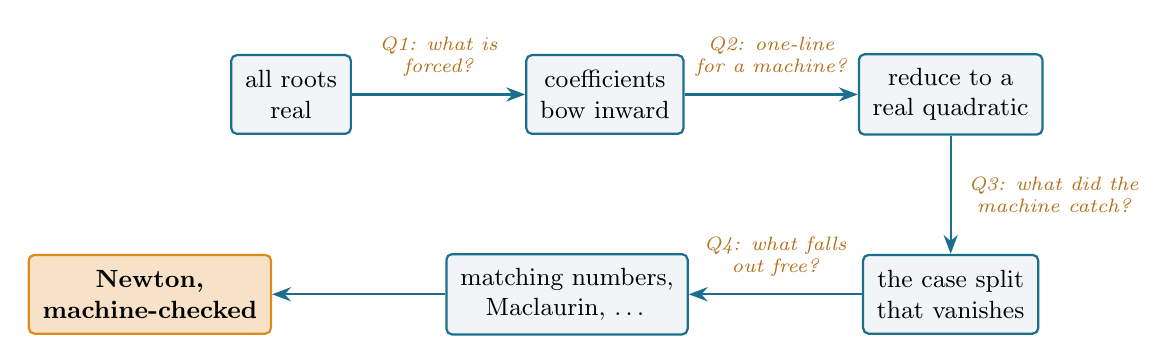
\begin{tikzpicture}[
  obj/.style={draw=ggteal,thick,rounded corners=2pt,fill=ggband!40,align=center,
    font=\small,inner sep=5pt,minimum height=10mm},
  q/.style={font=\scriptsize\itshape,text=ggamber!80!black,align=center},
  arr/.style={-{Stealth[length=2.4mm]},thick,ggteal}]
  \node[obj] (roots) {all roots\\real};
  \node[obj,right=22mm of roots] (bow) {coefficients\\bow inward};
  \node[obj,right=22mm of bow] (quad) {reduce to a\\real quadratic};
  \node[obj,below=15mm of quad] (caught) {the case split\\that vanishes};
  \node[obj,left=22mm of caught] (free) {matching numbers,\\Maclaurin, \dots};
  \node[obj,left=22mm of free,fill=ggamber!25,draw=ggamber] (done)
    {\textbf{Newton,}\\\textbf{machine-checked}};
  \draw[arr] (roots) -- node[q,above=1mm] {Q1: what is\\forced?} (bow);
  \draw[arr] (bow) -- node[q,above=1mm] {Q2: one-line\\for a machine?} (quad);
  \draw[arr] (quad) -- node[q,right=1mm] {Q3: what did the\\machine catch?} (caught);
  \draw[arr] (caught) -- node[q,above=1mm] {Q4: what falls\\out free?} (free);
  \draw[arr] (free) -- (done);
\end{tikzpicture}
\caption{The reader's map. From a hypothesis on the roots to a certified inequality and its
corollaries; each arrow is the question its section answers. Every node is a block of
\lean{sorry}-free Lean.}
\label{fig:readermap}
\end{figure}

\section{Q1: what does reality of the roots force on the coefficients?}\label{sec:intro}

Tell me nothing about a polynomial except that all of its roots are real---not where they are,
not whether they repeat---and I can already constrain its coefficients. That such a thing is
possible is mildly surprising; that the constraint is sharp, classical, and still doing heavy
lifting in today's combinatorics is the reason for this paper.

\emph{History bead.} The inequalities are Newton's, stated without proof in the
\emph{Arithmetica Universalis} (1707)~\cite{Newton1707}. Maclaurin (1729) deduced from them the
chain of mean inequalities that bears his name~\cite{Maclaurin1729}; a rigorous proof came only
in the nineteenth century (Sylvester), and the modern textbook account is
Hardy--Littlewood--P\'olya~\cite{HLP}. The mechanism---real-rootedness inherited by the
derivative (Rolle) and by the reversal of the polynomial---is the one formalized here.

Write a real-rooted polynomial through its roots, $p(x)=\sum_{k=0}^{n}(-1)^k e_k\,x^{n-k}$, where
$e_k$ is the $k$-th \emph{elementary symmetric function} of the roots, and form the
\emph{normalized means} $p_k=e_k/\binom{n}{k}$. Newton's claim is that the means are
\emph{log-concave}---each one at least the geometric mean of its neighbours. Three centuries on,
this is the cheapest instance of a pattern that organizes a large part of modern combinatorics:
to prove a sequence log-concave (hence unimodal, hence well-behaved), exhibit it as the
coefficients of a \emph{real-rooted} polynomial, and let Newton finish. The strategy underlies
Stanley's survey of log-concave sequences~\cite{Stanley1989}, Br\"and\'en's theory of stable
polynomials~\cite{Branden2015}, and---when no real-rooted polynomial is at hand---the deeper
Hodge-theoretic proof of Adiprasito--Huh--Katz that the characteristic polynomial of a matroid is
log-concave~\cite{AHK2018}. Newton's inequalities are the elementary, real-rooted floor of that
whole building.

\begin{theorem}[Newton's inequalities, in Lean~4; \lean{Newton.newton\_inequality}]
\label{thm:newton}
For a \emph{monic} real-rooted real polynomial $p$ of degree $n$ and every $1\le k\le n-1$,
\keyeq{e_k^2\,\binom{n}{k-1}\binom{n}{k+1}\;\ge\;e_{k-1}\,e_{k+1}\,\binom{n}{k}^{2}.}
Equivalently (\lean{newton\_logConcave}) the normalized means $p_k=e_k/\binom{n}{k}$ are
log-concave, $p_{k-1}\,p_{k+1}\le p_k^2$. Both are \lean{sorry}-free; \lean{\#print axioms} on
each reports only \lean{propext}, \lean{Classical.choice}, \lean{Quot.sound}.
\end{theorem}

The monic hypothesis loses nothing: the $e_k$ are symmetric functions of the roots alone, which
scaling does not move, so the inequality holds for \emph{every} real-rooted polynomial---and the
coefficient form \lean{newton\_inequality\_coeff} (Section~\ref{sec:proof}), the workhorse from
which this is derived, is machine-checked with no normalization at all.

\emph{Hand-checkable case.} Take $p(x)=(x-1)(x-2)(x-4)=x^3-7x^2+14x-8$, so $n=3$ and
$(e_0,e_1,e_2,e_3)=(1,7,14,8)$ (Figure~\ref{fig:bow}, left). At $k=1$ the theorem reads
$e_1^2\binom{3}{0}\binom{3}{2}=147\ge e_0e_2\binom{3}{1}^2=126$; at $k=2$, $588\ge504$. The
all-roots-equal polynomial $(x-1)^4$ \emph{saturates} every inequality (the sharp boundary), and
$x^2+1$---whose roots are not real---\emph{fails} it ($0\not\ge4$ at $k=1$), a reminder that the
hypothesis is load-bearing, not decorative (Figure~\ref{fig:bow}, right).

\begin{figure}[t]
\centering
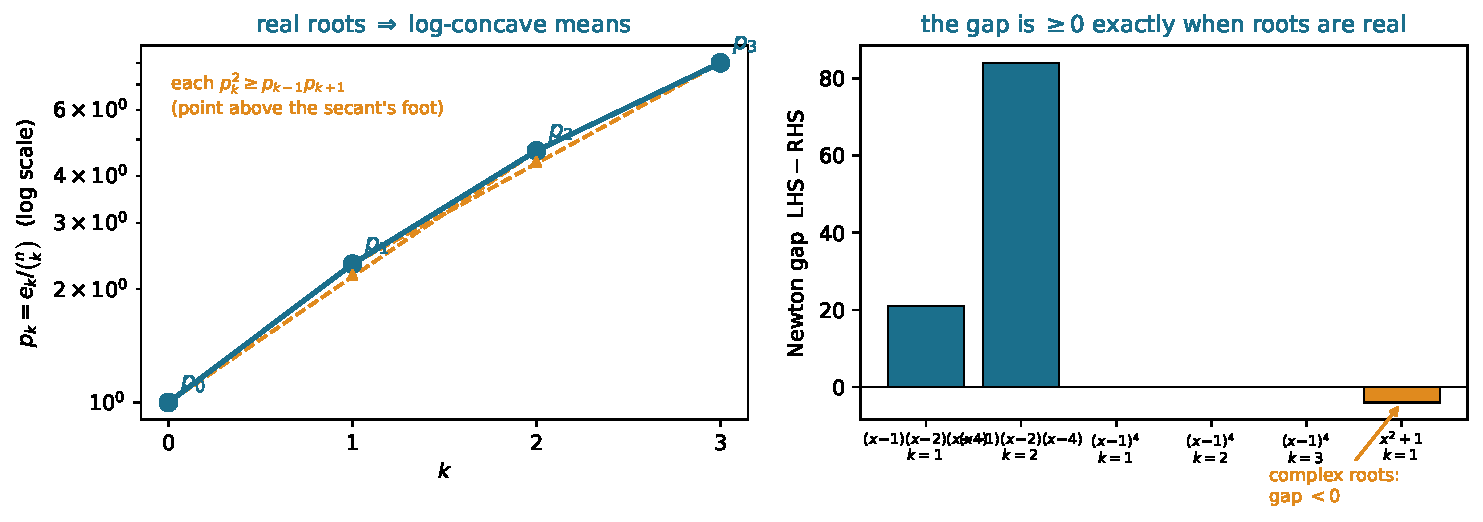
\includegraphics[width=0.92\textwidth]{newton_fig1_bow}
\caption{\emph{Left:} the normalized means of $(x-1)(x-2)(x-4)$, plotted on a log axis; each
interior mean sits above the geometric mean of its neighbours (the amber arrows), so the sequence
is concave---it ``bows inward.'' \emph{Right:} the Newton gap
$e_k^2\binom{n}{k-1}\binom{n}{k+1}-e_{k-1}e_{k+1}\binom{n}{k}^2$ at every interior $k$: positive
for the real-rooted cubic, exactly zero for $(x-1)^4$ (the sharp case), and \emph{negative} for
$x^2+1$. The generating script asserts every plotted value against exact integer arithmetic.}
\label{fig:bow}
\end{figure}

One feature of the statement repays a second look:
\begin{quote}\itshape
  why should the gap between real and complex roots surface precisely in the elementary symmetric
  functions, and precisely as log-concavity?
\end{quote}
Because the $e_k$ \emph{are} the coefficients of the polynomial, read through Vieta, and
real-rootedness is a property that propagates downward through the entire tower of derivatives
(Rolle) and survives reversing the polynomial. Those two moves let one isolate any three
consecutive coefficients as the coefficients of a real-rooted quadratic---and for a quadratic,
``real-rooted'' is literally ``discriminant $\ge0$.'' That is Newton's inequality, and the next
section is how a machine walks the same path. \emph{Can the textbook gesture become a one-line
check?}

\section{Q2: how do you make it a one-line check for a machine?}\label{sec:proof}

\emph{History bead.} The differentiation--reversal proof is the classical one (Sylvester; the
account in \cite{HLP}): grind the index down to a quadratic using operations that preserve reality
of roots, then invoke the trivial $n=2$ case. The whole question is whether ``preserves real
roots'' and ``reduce to a quadratic'' survive being made fully formal.

\paragraph{The objects.} I work over $\R$. A polynomial is \emph{real-rooted}
(\lean{RealRooted}) when it splits into linear factors over $\R$---Mathlib's intrinsic
\lean{Polynomial.Splits}; equivalently it has $\deg p$ real roots counted with multiplicity. For
the roots multiset $s=p.\mathtt{roots}$, the elementary symmetric function is
$e_k=\lean{Multiset.esymm}\,s\,k$, and $\binom{n}{k}=\lean{Nat.choose}$. Two pieces of Mathlib do
the bridging: \lean{coeff\_eq\_esymm\_roots\_of\_card} is Vieta,
$p.\mathtt{coeff}\,j=p.\mathtt{leadingCoeff}\cdot(-1)^{n-j}\,e_{n-j}$ (so I may pass between the
symmetric-function statement and a statement about coefficients), and
\lean{card\_roots\_le\_derivative} is Rolle for polynomials. Mathlib had both halves; it did not
have the inequality on them.

\paragraph{The two stones.} Exactly two operations preserve real-rootedness and that is all the
proof needs. \emph{Differentiation:} between consecutive real roots of $p$ lies a real root of
$p'$ (Rolle), so $p'$ has $\ge\deg p-1$ real roots, which is all it can have
(\lean{RealRooted.derivative}, iterated to \lean{RealRooted.iterate\_derivative}).
\emph{Reversal:} $p^{\mathrm{rev}}$ is, up to a nonzero factor, $p$ evaluated at $1/x$, so its
roots are the reciprocals of the nonzero roots of $p$, still real (\lean{RealRooted.reverse}).
With these, the reduction is short.

\begin{recipebox}{The reduction (recipe)}
To prove the inequality at index $i$ for a real-rooted $p$ of degree $n$ (set $N=n-i+1$):
(1)~differentiate $i-1$ times: $q=p^{(i-1)}$, real-rooted of degree $N$;
(2)~reverse: $r=q^{\mathrm{rev}}$, real-rooted;
(3)~differentiate $N-2$ times: $g=r^{(N-2)}$, real-rooted of degree $\le2$.
The three low coefficients of $g$ are \emph{factorial multiples} of $a_{i-1},a_i,a_{i+1}$ (writing
$a_j=p.\mathtt{coeff}\,j$), and the base case
$g.\mathtt{coeff}\,1^2\ge4\,g.\mathtt{coeff}\,2\cdot g.\mathtt{coeff}\,0$ is, after clearing those
positive factorials, Newton's inequality at $i$.
\end{recipebox}

\begin{figure}[t]
  \centering
  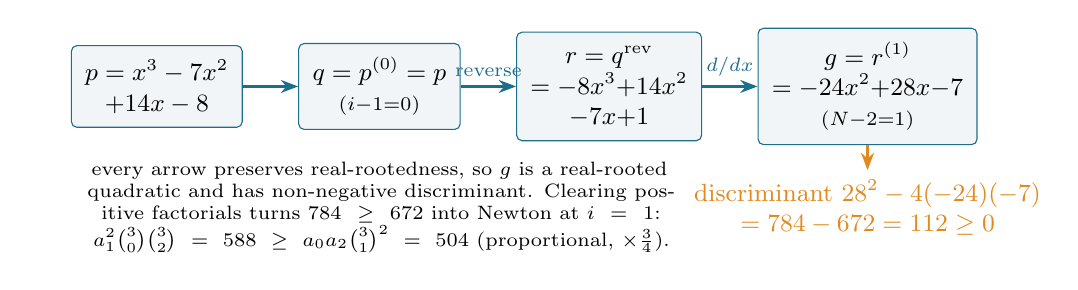
\begin{tikzpicture}[node distance=4pt,
    box/.style={draw=ggteal,fill=ggband!40,rounded corners=2pt,inner sep=5pt,align=center,font=\small},
    arr/.style={-{Stealth[length=2.2mm]},ggteal,thick}]
    \node[box] (p) {$p=x^3-7x^2$\\$+14x-8$};
    \node[box,right=20pt of p] (q) {$q=p^{(0)}=p$\\\scriptsize($i{-}1{=}0$)};
    \node[box,right=20pt of q] (r) {$r=q^{\mathrm{rev}}$\\$=-8x^3{+}14x^2$\\$-7x{+}1$};
    \node[box,right=20pt of r] (g) {$g=r^{(1)}$\\$=-24x^2{+}28x{-}7$\\\scriptsize($N{-}2{=}1$)};
    \draw[arr] (p) -- (q);
    \draw[arr] (q) -- (r) node[midway,above,font=\scriptsize,ggteal]{reverse};
    \draw[arr] (r) -- (g) node[midway,above,font=\scriptsize,ggteal]{$d/dx$};
    \node[below=9pt of g,align=center,font=\small,text=ggamber] (disc)
      {discriminant $28^2-4(-24)(-7)$\\$=784-672=112\ge0$};
    \draw[arr,ggamber] (g) -- (disc);
    \node[below=8pt of q,align=center,font=\scriptsize,text width=8.7cm] {%
      every arrow preserves real-rootedness, so $g$ is a real-rooted quadratic and has
      non-negative discriminant. Clearing positive factorials turns $784\ge672$ into Newton at
      $i=1$: $a_1^2\binom{3}{0}\binom{3}{2}=588\ge a_0a_2\binom{3}{1}^2=504$
      (proportional, $\times\tfrac34$).};
  \end{tikzpicture}
  \caption{The differentiate--reverse reduction, worked on the running cubic at $i=1$ (relating
  $a_0,a_1,a_2=-8,14,-7$). The final object is a quadratic; a real-rooted quadratic has
  non-negative discriminant; the factorials the proof cancels are the proportionality constant.}
  \label{fig:reduction}
\end{figure}

\paragraph{The base case, in coefficients.} The $n=2$ heart is \lean{realRooted\_discrim\_coeff}:
a real-rooted $q$ with $\deg q\le2$ satisfies $q.\mathtt{coeff}\,1^2\ge4\,q.\mathtt{coeff}\,2\cdot
q.\mathtt{coeff}\,0$. Evaluate $q$ at one of its roots $x$ and read off
$b^2-4ac=(2ax+b)^2-4a(ax^2+bx+c)=(2ax+b)^2\ge0$. Stating it on \emph{coefficients}, with the weak
hypothesis $\deg\le2$, is the choice that makes the whole proof clean (Section~\ref{sec:caught}).

\paragraph{The bookkeeping.} The one technical part is computing the three low coefficients of
$g$. Mathlib's \lean{coeff\_iterate\_derivative} gives $(p^{(k)}).\mathtt{coeff}\,m=
(m{+}k)^{\underline{k}}\,p.\mathtt{coeff}(m{+}k)$ (a falling factorial), and \lean{coeff\_reverse}
gives $q^{\mathrm{rev}}.\mathtt{coeff}\,m=q.\mathtt{coeff}(\mathrm{revAt}\,(\deg q)\,m)$.
Composing derivative--reverse--derivative needs the \emph{exact} degree of each intermediate,
which over $\R$ (characteristic zero, an \lean{IsAddTorsionFree} ring) is supplied by
\lean{degree\_derivative\_eq}: differentiating a degree-$d{>}0$ polynomial drops the degree by
exactly one. With degrees pinned, the discriminant inequality, after rewriting each falling
factorial through $\lean{Nat.factorial\_mul\_descFactorial}$, becomes
\keyeq{\bigl((N-1)!\,i!\bigr)^2\,a_i^2\;\ge\;N!\,(N-2)!\,(i-1)!\,(i+1)!\;a_{i-1}a_{i+1},}
and the binomial identity $\binom{n}{k}\,k!\,(n-k)!=n!$
(\lean{Nat.choose\_mul\_factorial\_mul\_factorial}) clears these positive factors to match
Theorem~\ref{thm:newton}---no inequality reasoning, only positivity. The symmetric-function form
then follows from the coefficient form (\lean{newton\_inequality\_coeff}) by Vieta, the signs
$(-1)^{k-1}(-1)^{k+1}=1$ cancelling and the binomials reindexing by
$\binom{n}{k}=\binom{n}{n-k}$ to the running index $i=n-k$.

So the answer to Q2 is yes: the inequality reduces, in three reality-preserving moves, to a single
discriminant a machine closes by \lean{sq\_nonneg}. \emph{And at the one place the textbook waves
its hand, the machine made me earn it.}

\section{Q3: what did the machine catch that the textbook glides over?}\label{sec:caught}

\emph{History bead.} ``Differentiate, reverse, reduce to a quadratic'' is how the classical proof
runs, and the classical proof quietly assumes the reversed polynomial keeps its degree. A proof
assistant does not let the assumption pass unexamined---and examining it removed a case split, not
added one.

The reversal step preserves \emph{degree} only when the reversed polynomial's leading coefficient
is nonzero, which fails exactly when $a_{i-1}=0$. The textbook reflex is a case split: handle
$a_{i-1}=0$ separately. I avoid it entirely, and the reason is the shape of the base case.

\begin{recipebox}{What a proof assistant earns its keep on}
Phrasing the base case on \emph{coefficients} with the weak hypothesis $\deg\le2$ (not $=2$) makes
it return a true statement even when the quadratic degenerates: if $g.\mathtt{coeff}\,2=0$ the
inequality reads $g.\mathtt{coeff}\,1^2\ge0$, which is \lean{sq\_nonneg}. Traced back, when
$a_{i-1}=0$ Newton's right-hand side is $a_{i-1}a_{i+1}\binom{n}{i}^2=0$ and the left-hand side is a
square times non-negative binomials---so the inequality holds for a reason unrelated to the
quadratic. \emph{The general machinery and the degenerate case are discharged by the same line.}
The transferable lesson: choosing the weakest honest hypothesis for a base case often dissolves the
edge cases a sharper statement would force you to chase.
\end{recipebox}

This is the whole of what the formalization added beyond transcription, and it is honestly
small---not a theorem but a discipline. It is also exactly the kind of step that justifies
machine-checking a result everyone already believes: the place where ``without loss of generality''
turns out to cost nothing, but only once you have looked. \emph{With Newton certified, what does
the rest of this line of work get for free?}

\section{Q4: with Newton certified, what falls out for free?}\label{sec:corollaries}

\emph{History bead.} The implication ``real-rooted $\Rightarrow$ log-concave coefficients'' is the
workhorse of the field: it is why the matching numbers of a graph are log-concave (via
Heilmann--Lieb~\cite{PartII}), why the coefficients of a claw-free graph's independence polynomial
are, and the easy half of the results that, for matroids, needed Hodge theory because no
real-rooted polynomial was available~\cite{AHK2018}.

The coefficient-form lemma \lean{newton\_inequality\_coeff} is stated precisely so that feeding it
any real-rooted polynomial yields log-concavity of that polynomial's coefficients, with no further
work:
\keyeq{\text{real-rooted}\;\Longrightarrow\;\text{log-concave coefficients}.}
The matching polynomial of a graph is real-rooted (Heilmann--Lieb, the previous paper in this
line~\cite{PartII}); composing it with the lemma proved here gives log-concavity of the matching
numbers as an immediate corollary, rather than the textbook gesture it has been throughout this
series. The same one line applies to any future real-rooted polynomial a Lean development produces.

Two roads open directly upward (Table~\ref{tab:inventory} lists what is built; these are what is
not yet):
\begin{itemize}\itemsep1pt
\item \textbf{Maclaurin's mean inequalities} $p_1\ge p_2^{1/2}\ge\cdots\ge p_n^{1/n}$, Newton's
  immediate historical consequence---now a concrete next target rather than a citation.
\item \textbf{The equality cases}: that equality at an interior $k$ forces all roots equal, the
  classical sharp companion, visible as the $(x-1)^4$ row of Figure~\ref{fig:bow} but not yet
  proved.
\end{itemize}

Here is a question worth carrying away:
\begin{quote}\itshape
  why should two operations as different as \emph{differentiating} and \emph{reciprocating the
  roots} both preserve reality of roots---and why is that pair exactly enough to expose every
  coefficient window?
\end{quote}
Because both are shadows of one fact: the real-rooted polynomials form a closed world (the
several-variable home is Br\"and\'en's stable polynomials~\cite{Branden2015}). Differentiation is
the simplest linear operator preserving it, reversal the simplest involution; between them they act
on coefficient windows transitively enough to surface any three consecutive coefficients as a
quadratic. Newton's inequalities are the first visible consequence of that closure---and the
reduction in this paper is, in miniature, how every later real-rootedness argument borrows its
strength.

\section{The building blocks}\label{sec:blocks}

The headline rests on four reusable pieces---the genuinely portable output---each \lean{sorry}-free
with the standard three axioms (Table~\ref{tab:inventory}).

\begin{lemma}[\lean{RealRooted.derivative}, \lean{RealRooted.iterate\_derivative}]
If $p$ is real-rooted then so is $p'$, and hence every iterated derivative $p^{(k)}$.
\end{lemma}
Rolle's theorem for polynomials (\lean{card\_roots\_le\_derivative}) squeezed against the degree
drop: $p'$ already has $\deg p-1$ real roots, which is the most it can have.

\begin{lemma}[\lean{RealRooted.reverse}]
If $p$ is real-rooted then so is its reversal $p^{\mathrm{rev}}$.
\end{lemma}
By factoring $p$ into monic linears and reversing each; the constant-term hypothesis the textbook
attaches is \emph{unnecessary} and is dropped---reversal merely discards trailing zeros, and the
remaining product of $\le1$-degree factors still splits.

\begin{lemma}[\lean{realRooted\_discrim\_coeff}]
A real-rooted $q$ with $\deg q\le2$ satisfies $q.\mathtt{coeff}\,1^2\ge4\,q.\mathtt{coeff}\,2\cdot
q.\mathtt{coeff}\,0$.
\end{lemma}
The base case of the reduction, in coefficient form; the source of the dissolved case split
(Section~\ref{sec:caught}).

\begin{table}[h]
\centering\small
\rowcolors{2}{ggband!35}{white}
\begin{tabular}{@{}lll@{}}
\toprule
\rowcolor{ggteal!18} Lean name & statement & role \\
\midrule
\lean{newton\_inequality} & $e_k^2\binom{n}{k-1}\binom{n}{k+1}\ge e_{k-1}e_{k+1}\binom{n}{k}^2$ & Theorem~\ref{thm:newton} \\
\lean{newton\_logConcave} & $p_{k-1}p_{k+1}\le p_k^2$ (normalized means) & corollary \\
\lean{newton\_inequality\_coeff} & $a_i^2\binom{n}{i-1}\binom{n}{i+1}\ge a_{i-1}a_{i+1}\binom{n}{i}^2$ & coefficient form \\
\lean{realRooted\_discrim\_coeff} & real-rooted, $\deg\le2\Rightarrow a_1^2\ge4a_2a_0$ & base case \\
\lean{RealRooted.derivative} & $p$ real-rooted $\Rightarrow p'$ real-rooted & block (Rolle) \\
\lean{RealRooted.iterate\_derivative} & $p$ real-rooted $\Rightarrow p^{(k)}$ real-rooted & block \\
\lean{RealRooted.reverse} & $p$ real-rooted $\Rightarrow p^{\mathrm{rev}}$ real-rooted & block \\
\bottomrule
\end{tabular}
\caption{The load-bearing results, all \lean{sorry}-free in \lean{Newton.lean} of the repository
(346 lines, on \lean{RealStable.lean} and Mathlib). Axioms of every entry: \lean{propext},
\lean{Classical.choice}, \lean{Quot.sound} only; no \lean{native\_decide}, no custom axiom.}
\label{tab:inventory}
\end{table}

\section{The boundary of the contribution}\label{sec:boundary}

Everything here that is mathematics is classical: Newton (1707), Maclaurin (1729), Sylvester's
proof, the textbook treatment in Hardy--Littlewood--P\'olya~\cite{HLP}. I claim no new identity and
no new inequality. The contributions are three: the \emph{formalization} (to my knowledge the first
machine-checked proof of Newton's inequalities in any proof assistant); the \emph{reusable
infrastructure}---real-rootedness under differentiation, iterated differentiation, and reversal,
and the coefficient-form discriminant---which is exactly what any further real-rootedness or
stability development in Mathlib will want; and the \emph{proof-engineering record} of
Section~\ref{sec:caught}, the weak-hypothesis base case that dissolves a case split.

\emph{Scope, stated plainly.} I prove the inequalities \emph{over $\R$}---the natural home of
real-rootedness, and what the reduction uses---not over an abstract real-closed or ordered field,
though nothing in the argument resists it. I prove the inequality and its log-concave corollary,
\emph{not} the equality/strictness analysis (equality forces all roots equal), and not Maclaurin's
mean chain: those are mapped (Section~\ref{sec:corollaries}), not built.

\emph{Prior formalizations.} The priority claim rests on a documented search, not a feeling. For
Newton's inequalities and the elementary symmetric functions I searched (June~2026): Mathlib
(Loogle and \lean{grep}---\lean{Multiset.esymm} and the Vieta relations exist; \emph{Maclaurin} and
\lean{esymm}-squared inequalities do not), the wider Lean community repositories, the Isabelle
Archive of Formal Proofs, and the Coq/Rocq ecosystem. None contains Newton's inequalities. As
always, such a claim is made to the best of my knowledge.

\emph{On methodology.} The formalization was done with an AI assistant (Claude, Anthropic), under
the discipline of the companion papers: the reduction's arithmetic verified numerically before
formalizing (\lean{figures/newton\_fig1\_bow.py} re-checks every instance), and every named theorem
verified by \lean{\#print axioms} to depend only on \lean{propext}, \lean{Classical.choice},
\lean{Quot.sound}. Correctness does not rest on the assistant: the Lean kernel checks every proof.
The careful accounting---the scope over $\R$ stated as plainly as the result, the equality cases
left explicitly open---is itself part of what the method, at its best, should produce. The
mathematics and the claims are the author's responsibility.

\section{Open questions}\label{sec:questions}

Newton's inequalities are now a theorem in the library. The concrete next targets---Maclaurin's
mean chain, the equality cases, log-concavity of the matching numbers---are named in
Section~\ref{sec:corollaries}; what follows are the questions I would rather carry away than tick
off, one per turn of the argument, the last one the one to keep.

\begin{enumerate}
\item \emph{Why zeros become magnitudes.} Reality of the roots is a statement about \emph{where} a
polynomial vanishes; log-concavity is a statement about the \emph{size} of its coefficients. Newton
is the first and cheapest bridge between the two. What is the deepest reason a constraint on a
polynomial's zeros should turn, window by window, into a constraint on the magnitude of its
coefficients?
\item \emph{The certificate hierarchy.} For a sequence of non-negative reals, real-rootedness of the
generating polynomial is equivalent to being a P\'olya frequency sequence
(Aissen--Schoenberg--Whitney), strictly stronger than log-concavity (which is $\mathrm{PF}_2$).
Newton derives the weak end from the strong. What exactly lives in the gap between the rungs, and is
there a \emph{cheapest} certificate for each that a proof assistant could be taught to choose?
\item \emph{The closure, made explicit.} Differentiation and reversal each preserve
real-rootedness, and that pair alone already exposes any three consecutive coefficients as a
quadratic. What is the full monoid of real-rootedness-preserving operations on coefficient windows,
and is ``reaches every quadratic window'' a theorem one could state and check---i.e.\ is the
sufficiency of \emph{these two} stones itself a theorem?
\item \emph{Above the real-rooted floor.} Where no real-rooted polynomial exists---matroids---%
log-concavity needs Hodge theory~\cite{AHK2018}, with Br\"and\'en's Lorentzian polynomials
interpolating between the two worlds. Is Newton the one-variable shadow of Lorentzian-ness, and what
is the smallest formalized fragment that would make it one storey of a single building rather than an
isolated classical fact?
\item \emph{One to keep.} The only thing formalizing added beyond transcription was that the
\emph{weakest honest} base-case hypothesis dissolved a case split
(Section~\ref{sec:caught})---``without loss of generality'' cost nothing, but only once a machine
made me look. In a theory three centuries old and re-proved many times, how often is the WLOG
genuinely free, and is ``always reach for the weakest base hypothesis'' a transferable principle of
machine proof or a happy accident of this one?
\end{enumerate}

\section*{Reproducing}
\begin{verbatim}
git clone https://github.com/karlesmarin/godsil-gutman-lean
cd godsil-gutman-lean && lake exe cache get
lake env lean Newton.lean
\end{verbatim}
Lean \lean{v4.30.0-rc2}, Mathlib pin \lean{701fb6e9}. The theorems are
\lean{Newton.newton\_inequality}, \lean{newton\_logConcave} and \lean{newton\_inequality\_coeff} in
\lean{Newton.lean}; their supports are in Table~\ref{tab:inventory}. Each is checked by
\lean{\#print axioms} to depend only on \lean{propext}, \lean{Classical.choice}, \lean{Quot.sound}.
The figure regenerates with \lean{python figures/newton\_fig1\_bow.py}, which asserts its content
against exact arithmetic before drawing.

\begin{thebibliography}{99}\small
\bibitem{Newton1707} I.~Newton, \emph{Arithmetica Universalis} (1707); the inequalities among the
coefficients of a polynomial with real roots are stated there without proof.
\bibitem{Maclaurin1729} C.~Maclaurin, A second letter \dots\ concerning the roots of equations,
with the demonstration of other rules in algebra, \emph{Phil.\ Trans.\ Roy.\ Soc.\ London}
\textbf{36} (1729) 59--96.
\bibitem{HLP} G.~H.~Hardy, J.~E.~Littlewood, G.~P\'olya, \emph{Inequalities}, 2nd ed., Cambridge
Univ.\ Press, 1952 (Newton's and Maclaurin's inequalities, \S2.22).
\bibitem{Stanley1989} R.~P.~Stanley, Log-concave and unimodal sequences in algebra,
combinatorics, and geometry, \emph{Ann.\ New York Acad.\ Sci.} \textbf{576} (1989) 500--535.
\bibitem{Branden2015} P.~Br\"and\'en, Unimodality, log-concavity, real-rootedness and beyond, in
\emph{Handbook of Enumerative Combinatorics}, CRC Press, 2015, 437--483.
\bibitem{AHK2018} K.~Adiprasito, J.~Huh, E.~Katz, Hodge theory for combinatorial geometries,
\emph{Ann.\ of Math.} \textbf{188} (2018) 381--452.
\bibitem{PartI} C.~Mar\'in, \emph{Random Signs into Matchings: A Godsil--Gutman Identity,
Formalized in Lean~4}, Zenodo, 2026. \texttt{doi:10.5281/zenodo.20517350}.
\bibitem{PartII} C.~Mar\'in, \emph{Unfolding a Graph into a Tree: A Machine-Checked Proof of the
Heilmann--Lieb Theorem in Lean~4}, Zenodo, 2026.
\texttt{https://github.com/karlesmarin/godsil-gutman-lean}.
\bibitem{Mathlib2020} The mathlib Community, The Lean mathematical library, in \emph{CPP 2020},
ACM, 2020, 367--381.
\end{thebibliography}

\end{document}
